\documentclass{report}

\input{latex-templates/preamble}
\newcommand{\eps}{\epsilon}
\newcommand{\veps}{\varepsilon}
\newcommand{\Qed}{\begin{flushright}\qed\end{flushright}}

\newcommand{\parinn}{\setlength{\parindent}{1cm}}
\newcommand{\parinf}{\setlength{\parindent}{0cm}}

% \newcommand{\norm}{\|\cdot\|}
\newcommand{\inorm}{\norm_{\infty}}
\newcommand{\opensets}{\{V_{\alpha}\}_{\alpha\in I}}
\newcommand{\oset}{V_{\alpha}}
\newcommand{\opset}[1]{V_{\alpha_{#1}}}
\newcommand{\lub}{\text{lub}}
\newcommand{\del}[2]{\frac{\partial #1}{\partial #2}}
\newcommand{\Del}[3]{\frac{\partial^{#1} #2}{\partial^{#1} #3}}
\newcommand{\deld}[2]{\dfrac{\partial #1}{\partial #2}}
\newcommand{\Deld}[3]{\dfrac{\partial^{#1} #2}{\partial^{#1} #3}}
\newcommand{\der}[2]{\frac{\mathrm{d} #1}{\mathrm{d} #2}}
% \newcommand{\ddd}[3]{\frac{\mathrm{d}^{#3} #1}{\mathrm{d}^{#3} #2}}
\newcommand{\lm}{\lambda}
\newcommand{\uin}{\mathbin{\rotatebox[origin=c]{90}{$\in$}}}
\newcommand{\usubset}{\mathbin{\rotatebox[origin=c]{90}{$\subset$}}}
\newcommand{\lt}{\left}
\newcommand{\rt}{\right}
\newcommand{\bs}[1]{\boldsymbol{#1}}
\newcommand{\exs}{\exists}
\newcommand{\st}{\strut}
\newcommand{\dps}[1]{\displaystyle{#1}}
\newcommand{\id}{\text{id}}
\newcommand{\imps}{\quad \Rightarrow \quad}
\newcommand{\cimps}{\quad \Leftrightarrow \quad}
\newcommand{\kyuki}[1]{\quad \quad \bqty{\because \eqref{#1}}}
\newcommand{\kyukifir}[2]{\quad \quad \bqty{\because \eqref{#1} \& \eqref{#2}}}
\newcommand{\boxdia}[2]{\begin{wrapfigure}{r}{#1\textwidth}
		\fbox{\includegraphics[width=\linewidth]{Figures/#2.png}}
	\end{wrapfigure}}
\newcommand{\dia}[2]{\begin{wrapfigure}{r}{#1\textwidth}
		\includegraphics[width=\linewidth]{Figures/#2.png}
	\end{wrapfigure}}
\newcommand{\boxudia}[2]{\begin{figure}[H]
		\centering
		\fbox{\includegraphics[width=#1\textwidth]{Figures/#2.png}}
		\end{figure}}
\newcommand{\udia}[2]{\begin{figure}[H]
		\centering
		\includegraphics[width=#1\textwidth]{Figures/#2.png}
	\end{figure}}
\newcommand{\su}[2]{\textcolor{my#1}{#2}}
\newcommand{\shs}[1]{\\ \textbf{{\Large #1}}\\}
\newcommand{\sss}[1]{\vspace*{-1cm} \subsubsection*{#1}}
\newcommand{\unt}[1]{\text{#1}}
\newcommand{\wa}{
	\noindent\rule{\textwidth}{0.4pt} 
	\vspace{0.5cm}}
\newcommand{\wb}{\noindent\rule{\textwidth}{0.4pt}}
\newcommand{\qmi}{\int_{-\infty}^{\infty}}
\newcommand{\qmk}{|\psi(x,0)|^{2}}
\newcommand{\qml}{\exp{-\frac{(x - x_0)^2}{4\sigma_0^2} + \frac{i}{\hbar}p_0 x}}
\newcommand{\qmls}{\exp{-\frac{(x - x_0)^2}{4\sigma_0^2} - \frac{i}{\hbar}p_0 x}}
\newcommand{\e}[1]{\exp\lt(#1\rt)}
\newcommand\prm[2][^n]{\prescript{#1\mkern-2.5mu}{}P_{#2}}
\newcommand\cmb[2][^n]{\prescript{#1\mkern-0.5mu}{}C_{#2}}
\newcommand{\ki}[1]{\lt[\therefore #1\rt]}
\newcommand{\h}{\underset{\rotatebox{135}{\#}}{}}
\newcommand{\f}{\frac{1}{2}}


%\newcommand{\sol}[1]{\vspace{0.5cm} 
%\setlength{\parindent}{0cm} \textcolor{mytheoremfr}{\textbf{\underline{Solution:}}} \textcolor{mytheoremfr}{#1}}
\newcommand{\solve}[1]{\setlength{\parindent}{0cm}\textbf{\textit{Solution: }}\setlength{\parindent}{1cm}#1 \Qed}

\input{latex-templates/letterfonts}
\usepackage{physics}
\usepackage{float}
\usepackage{tikz}
\usetikzlibrary{decorations.pathreplacing}

\title{\Huge{Undergraduate Physics}\\ Personal Notes }
\author{\huge{Parth Bhargava}}
\date{}

\begin{document}
	
	\maketitle
	\newpage% or \cleardoublepage
	% \pdfbookmark[<level>]{<title>}{<dest>}
	\pdfbookmark[section]{\contentsname}{toc}
	\tableofcontents
	\pagebreak
	
	\chapter{Single-Variable Calculus}
	\chapter{Newtonian Mechanics}
	\section{Kinematics}
	
	$$ \avg{\va{v}} = \frac{\va{r_2}-\va{r_1}}{t_2-t_1} = \frac{\Delta \va{r}}{\Delta t} \imps \va{v} = \dv{\va{r}}{t} = \int \va{a}.\dd t \qc \avg{\va{a}} = \frac{\va{v_2}-\va{v_1}}{t_2-t_1} = \frac{\Delta \va{v}}{\Delta t} \imps \va{a} = \dv{\va{v}}{t} = \dv[2]{\va{r}}{t} = \va{v}\dv{\va{v}}{\va{r}} $$\\[1pt]
	
	\mprop{}{Under constant $\va{a}$; 
	$$\va{v}=\va{u}+\va{a}t \qc \va{s}=\va{u}t+\frac{1}{2}\va{a}t^2 \qc v^2=u^2 +2as \qc s_n=u+\frac{1}{2}a(2n-1)$$
	Constant $\va{a}$ can be identified as when,
	$$v \propto \sqrt{x} \qc v \propto t \qc x \propto t^2$$ 
	}
	
	\ex{Projectile Motion}{
	Equations for a general case of projectile motion,
	$$T_f=\frac{2u_y}{a_y} \quad
	H=\frac{u_y^2}{2a_y} \quad R=u_xT_f+\frac{1}{2}a_xT_f^2$$
	
	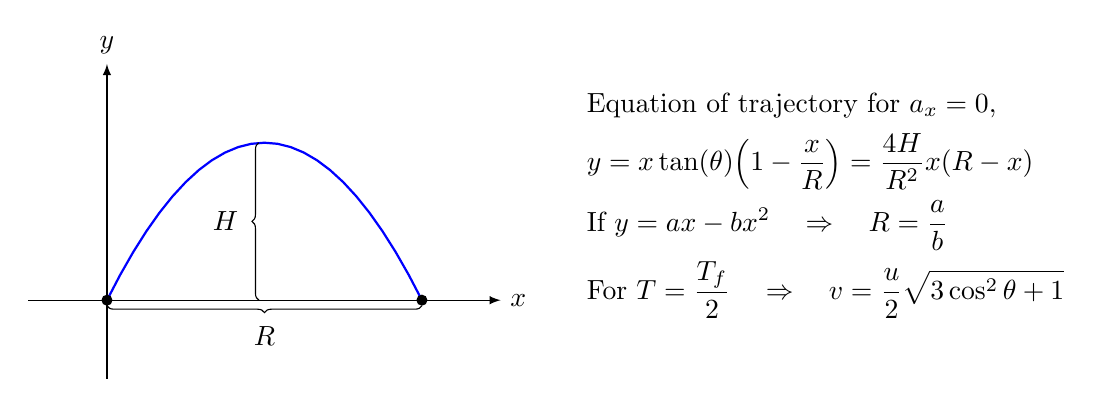
\begin{tikzpicture}[>=latex]
		\def\R{4} % Range
		\def\H{2} % Maximum height
		
		% Coordinate axes
		\draw[->] (-1,0) -- (\R+1,0) node[right] {$x$};
		\draw[->] (0,-1) -- (0,\H+1) node[above] {$y$};
		
		% Projectile path (parabola)
		\draw[blue, thick] plot[domain=0:\R] (\x, {-\H*4/(\R*\R)*\x*(\x - \R)});
		
		% Labels for range and height
		\draw[decorate, decoration={brace, mirror, raise=2pt}] (0,0) -- (\R,0) 
		node[midway, below=6pt] {$R$};
		\draw[decorate, decoration={brace, raise=2pt}] (\R/2,0) -- (\R/2,\H) 
		node[midway, left=6pt] {$H$};
		
		% Start/end points
		\fill (0,0) circle (2pt);
		\fill (\R,0) circle (2pt);
		
		% Equations on the right (key projectile motion formulas)
		\node[anchor=west] at ([xshift=15pt]current bounding box.east) {%
			$\begin{aligned}
				&\text{Equation of trajectory for $a_x=0$,} \\ 
				&y=x\tan(\theta)\pqty{1-\frac{x}{R}}=\frac{4H}{R^2}x(R-x)\\
				&\text{If } y=ax-bx^2 \imps R=\frac{a}{b}\\
				&\text{For } T=\frac{T_f}{2} \imps \avg{v}=\frac{u}{2}\sqrt{3\cos^2{\theta}+1}\\
			\end{aligned}$%
		};
		
	\end{tikzpicture}
	}
	\mprop{}{Analyse motion along each co-ordinate axis independently and superpose}
	\pagebreak
	Relative velocity of A with respect to B,
	$$v_{AB}=\frac{v_A-v_B}{1-\frac{v_Av_B}{c^2}} \imps v_{AB} \approx v_A - v_B$$
	\ex{Projectile on a trolley moving with velocity $v_T$}{
	$$T_f=\frac{2u_y}{a_y} \quad
	H=\frac{u_y^2}{2a_y} \quad R=\pqty{u_x+v_T}T_f+\frac{1}{2}a_xT_f^2$$
	}
	\ex{Converging Polygon}{$$t=\frac{a}{v\pqty{1-\cos{\frac{2\pi}{n}}}}$$
	}
	\ex{Shortest distance Problem}{To calculate the shortest distance between two moving bodies A and B,
	}
	\ex{Chasing Problem}{
		\begin{align*}
			&T=\frac{l\pqty{v+u\sin{\theta}}}{v^2 - u^2}\\
			&\text{For $v=u$ we get,}\\
			&r_{min}=\frac{l}{2}\pqty{1+\sin{\theta}}
		\end{align*}
	}
	\mprop{}{For a particle moving at constant speed with rotating $\va{v}$,$$v_f-v_i=2v_0\sin{\frac{\dd{\beta}}{2}} \approx v_0\dd{\beta} \imps \va{a} = v_0 \dv{\beta}{t}=v_0\omega $$}
	\ex{Rain-Man Problems}{mr}
	\ex{River-Swimmer Problems}{dd}
	\section{Newton's Laws of Motion}
	cdf
	\section{Work and Energy}
	\section{Momentum and Collision}
	\chapter{Rigid Body Mechanics}
	\section{Rotation of Rigid Bodies}
	\section{Rotational Dynamics}
	\chapter{Gravitation}
	\chapter{Oscillation and Waves}
	\chapter{Lagrangian Mechanics}
	We begin by carefully considering generalized coordinates.
	\begin{itemize}
		\item Consider a system with Cartesian coordinates $x_A$. Hamilton’s principle, also called the principle of least action, states that solutions of the equations of motion are critical points of the action $S = \int L \dd t$ for fixed endpoints $q(t_i)$ and $q(t_f)$. This implies the Euler–Lagrange equation $$\dv{t}\pdv{L}{\dot{x}}=\pdv{L}{x}$$where we have dropped indices for simplicity. Here, we have $L=L(x,\dot{x})$ and the partial derivative is defined by holding all other arguments of the function constant. 
		\item It follows directly from the chain rule that the Euler–Lagrange equations are preserved by any invertible coordinate change, to generalized coordinates $q_a = q_a(x_A)$, because the action is a property of a path and hence is extremized regardless of the coordinates used to describe the path. The ability to use any generalized coordinates we want is a key practical advantage of Lagrangian mechanics over Newtonian mechanics.
	\end{itemize}
	
	\chapter{Multi-Variable Calculus}
	\chapter{Fluid Dynamics}
	\chapter{Electromagnetism}
	\sss{Maxwell's Equations:}
	\begin{align*}
		\divergence \vb{E} &= \frac{1}{\epsilon_0} \rho &&
		\curl \vb{E} = -\pdv{\vb{B}}{t} \\
		\divergence \vb{B} &= 0 &&
		\curl \vb{B} = \mu_0 \vb{J} + \mu_0 \epsilon_0 \pdv{\vb{E}}{t}
	\end{align*}
	
	\sss{Potentials:}
	\begin{align*}
		\vb{E} = -\grad V - \pdv{\vb{A}}{t} && \vb{B} = \curl \vb{A}
	\end{align*}
	
	\sss{Lorentz force law:}
	\begin{align*}
		\vb{F} = q (\vb{E} + \vb{v} \times \vb{B})
	\end{align*}
	
	\chapter{Quantum Mechanics}
	\section{The Wave Function}
	
	\begin{itemize}
		\item For the position representation of the wave function $\Psi(x,t)$ and the momentum representation of wave function $\Phi(x,t)$,
		$$\Psi(x,t)=\frac{1}{\sqrt{2\pi\hbar}}\int_{-\infty}^\infty\Phi(p,t)\exp\left(\frac{i}{\hbar}px\right)dp \cimps \Phi(p,t)=\frac{1}{\sqrt{2\pi\hbar}}\int_{-\infty}^\infty\Psi(x,t)\exp\left(-\frac{i}{\hbar}px\right)dx \\$$
		\clm{The Schrödinger Equation and Probability Density Function}{}{
			\begin{table}[H]
				\centering
				\def\arraystretch{2.5}	
				\begin{tabular}{||c||c||c||}
					\hline
					$\Psi$ & $\dps{i\hbar\pdv{\Psi}{t}=\frac{-\hbar^2}{2m}\pdv[2]{\Psi}{x} + V\Psi}$ & $\dps{\int_{a}^{b}|\Psi|^2.\dd x =P[a \leq x(t) \leq b] \imps \int_{-\infty}^{\infty}|\Psi|^2.\dd x =1}$ \\ \hline
					$\Phi$ & $\dps{i\hbar\pdv{\Phi}{t}=\frac{p^2}{2m}\Phi + V\pqty{i\hbar\pdv{p}}\Phi}$ & $\dps{\int_{a}^{b}|\Phi|^2.\dd p =P[a \leq p(t) \leq b] \imps \int_{-\infty}^{\infty}|\Phi|^2.\dd p =1}$ \\ \hline
				\end{tabular}
			\end{table}
		}
		\item Expectation value of quantity $Q$ is, $$\avg{Q\pqty{x,-i\hbar \pdv{x}}}= \int_{-\infty}^{\infty} \Psi^{*} [Q] \Psi .\dd x$$
		For example, 
		$$\avg{p}= \int_{-\infty}^{\infty} \Psi^{*} \bqty{i\hbar \pdv{x}} \Psi .\dd x \quad , \quad \avg{x}= \int_{-\infty}^{\infty} \Psi^{*} [x] \Psi .\dd x$$
		\thm{Erhenfest's Theorem}{
			Expectation values obey classical laws.
			$$\dv{t} \avg{p} = \avg{-V' (x)} \quad , \quad \dv{t} \avg{x} = \frac{1}{m} \avg{p} \ldots $$
		}
		\item Using the Normalisation condition we can derive the continuity equation in quantum mechanics as follows,
		$$\dv{t}\int_{-\infty}^{\infty} \Psi^{*} \Psi .\dd x =0 \imps \pdv{t}\rho(x,t)+\pdv{x}j(x,t)=0$$
		with probability density funcition associated with $x$
		$$\rho(x,t)\equiv|\Psi(x,t)|^2$$
		and the corresponding probability current density function
		$$j(x,t)\equiv\frac{1}{2m}\left\{\Psi^*(x,t)\left(-i\hbar\pdv{x}\right)\Psi(x,t)+\left[\left(-i\hbar\pdv{x}\right)\Psi(x,t)\right]^*\Psi(x,t)\right\}$$
		In terms of $j(x,t)$,
		$$\dv{t}\int_{x_1}^{x_2}\rho(x,t)dx=\int_{x_1}^{x_2}\pdv{t}\rho(x,t)\dd x=-\int_{x_1}^{x_2}\pdv{x}j(x,t)dx=-[j(x_2,t)-j(x_1,t)]$$
	\end{itemize}
	
	\chapter{Appendix}
	
	\begin{align*}
		\epsilon_0 &= 8.85 \times 10^{-12} \, \text{C}^2/\text{N}\text{m}^2 & (\text{permittivity of free space}) \\
		\mu_0 &= 4\pi \times 10^{-7} \, \text{N}/\text{A}^2 & (\text{permeability of free space}) \\
		c &= 3.00 \times 10^{8} \, \text{m/s} & (\text{speed of light}) \\
		e &= 1.60 \times 10^{-19} \, \text{C} & (\text{charge of the electron}) \\
		m &= 9.11 \times 10^{-31} \, \text{kg} & (\text{mass of the electron}) \\
		m_p &= 1.67 \times 10^{-27} \, \text{kg} & (\text{mass of proton})
	\end{align*}
	
	\section{Vector Calculus}
	\subsection{Cartesian Coordiantes}
	\begin{align*}
		\dd{\vb{l}} &= \dd{x} \vu*{x} + \dd{y} \vu*{y} + \dd{z} \vu*{z}; \quad \dd{\tau} = \dd{x} \dd{y} \dd{z} \\
		\text{\underline{Gradient:}} \quad \grad t &= \pdv{t}{x} \vu*{x} + \pdv{t}{y} \vu*{y} + \pdv{t}{z} \vu*{z} \\
		\text{\underline{Divergence:}} \quad \divergence \vb{v} &= \pdv{v_x}{x} + \pdv{v_y}{y} + \pdv{v_z}{z} \\
		\text{\underline{Curl:}} \quad \curl \vb{v} &= \left( \pdv{v_z}{y} - \pdv{v_y}{z} \right) \vu*{x} + \left( \pdv{v_x}{z} - \pdv{v_z}{x} \right) \vu*{y} + \left( \pdv{v_y}{x} - \pdv{v_x}{y} \right) \vu*{z} \\
		\text{\underline{Laplacian:}} \quad \laplacian t &= \pdv[2]{t}{x} + \pdv[2]{t}{y} + \pdv[2]{t}{z}
	\end{align*}
	
	\subsection{Spherical Coordinates}
	\begin{align*}
		\left\{
		\begin{aligned}
			x &= r \sin\theta \cos\phi \\
			y &= r \sin\theta \sin\phi \\
			z &= r \cos\theta
		\end{aligned}
		\right.
		&&
		\left\{
		\begin{aligned}
			\vu*{x} &= \sin\theta \cos\phi \vu*{r} + \cos\theta \cos\phi \vu*{\theta} - \sin\phi \vu*{\phi} \\
			\vu*{y} &= \sin\theta \sin\phi \vu*{r} + \cos\theta \sin\phi \vu*{\theta} + \cos\phi \vu*{\phi} \\
			\vu*{z} &= \cos\theta \vu*{r} - \sin\theta \vu*{\theta}
		\end{aligned}
		\right.
	\end{align*}
	\begin{align*}
		\left\{
		\begin{aligned}
			r &= \sqrt{x^2 + y^2 + z^2} \\
			\theta &= \tan^{-1}(\sqrt{x^2 + y^2}/z) \\
			\phi &= \tan^{-1}(y/x)
		\end{aligned}
		\right.
		&&
		\left\{
		\begin{aligned}
			\vu*{r} &= \sin\theta \cos\phi \vu*{x} + \sin\theta \sin\phi \vu*{y} + \cos\theta \vu*{z} \\
			\vu*{\theta} &= \cos\theta \cos\phi \vu*{x} + \cos\theta \sin\phi \vu*{y} - \sin\theta \vu*{z} \\
			\vu*{\phi} &= -\sin\phi \vu*{x} + \cos\phi \vu*{y}
		\end{aligned}
		\right.
	\end{align*}
	\begin{align*}
		\dd{\vb{l}} &= \dd{r} \vu*{r} + r \dd{\theta} \vu*{\theta} + r \sin\theta \dd{\phi} \vu*{\phi}; \quad \dd{\tau} = r^2 \sin\theta \dd{r} \dd{\theta} \dd{\phi} \\
		\text{\underline{Gradient:}} \quad \grad t &= \pdv{t}{r} \vu*{r} + \frac{1}{r} \pdv{t}{\theta} \vu*{\theta} + \frac{1}{r \sin\theta} \pdv{t}{\phi} \vu*{\phi} \\
		\text{\underline{Divergence:}} \quad \divergence \vb{v} &= \frac{1}{r^2} \pdv{(r^2 v_r)}{r} + \frac{1}{r \sin\theta} \pdv{(\sin\theta v_\theta)}{\theta} + \frac{1}{r \sin\theta} \pdv{v_\phi}{\phi} \\
		\text{\underline{Curl:}} \quad \curl \vb{v} &= \frac{1}{r \sin\theta} \left[ \pdv{(\sin\theta v_\phi)}{\theta} - \pdv{v_\theta}{\phi} \right] \vu*{r} \\
		&\quad + \frac{1}{r} \left[ \frac{1}{\sin\theta} \pdv{v_r}{\phi} - \pdv{(r v_\phi)}{r} \right] \vu*{\theta} + \frac{1}{r} \left[ \pdv{(r v_\theta)}{r} - \pdv{v_r}{\theta} \right] \vu*{\phi} \\
		\text{\underline{Laplacian:}} \quad \laplacian t &= \frac{1}{r^2} \pdv{}{r} \left( r^2 \pdv{t}{r} \right) + \frac{1}{r^2 \sin\theta} \pdv{}{\theta} \left( \sin\theta \pdv{t}{\theta} \right) + \frac{1}{r^2 \sin^2\theta} \pdv[2]{t}{\phi}
	\end{align*}
	
	\subsection{Cylindrical Coordinates}
	\begin{align*}
		\left\{
		\begin{aligned}
			x &= s \cos\phi \\
			y &= s \sin\phi \\
			z &= z
		\end{aligned}
		\right.
		&&
		\left\{
		\begin{aligned}
			\vu*{x} &= \cos\phi \vu*{s} - \sin\phi \vu*{\phi} \\
			\vu*{y} &= \sin\phi \vu*{s} + \cos\phi \vu*{\phi} \\
			\vu*{z} &= \vu*{z}
		\end{aligned}
		\right.
	\end{align*}
	\begin{align*}
		\left\{
		\begin{aligned}
			s &= \sqrt{x^2 + y^2} \\
			\phi &= \tan^{-1}(y/x) \\
			z &= z
		\end{aligned}
		\right.
		&&
		\left\{
		\begin{aligned}
			\vu*{s} &= \cos\phi \vu*{x} + \sin\phi \vu*{y} \\
			\vu*{\phi} &= -\sin\phi \vu*{x} + \cos\phi \vu*{y} \\
			\vu*{z} &= \vu*{z}
		\end{aligned}
		\right.
	\end{align*}
	\begin{align*}
		\dd{\vb{l}} &= \dd{s} \vu*{s} + s \dd{\phi} \vu*{\phi} + \dd{z} \vu*{z}; \quad \dd{\tau} = s \dd{s} \dd{\phi} \dd{z} \\
		\text{\underline{Gradient:}} \quad \grad t &= \pdv{t}{s} \vu*{s} + \frac{1}{s} \pdv{t}{\phi} \vu*{\phi} + \pdv{t}{z} \vu*{z} \\
		\text{\underline{Divergence:}} \quad \divergence \vb{v} &= \frac{1}{s} \pdv{(s v_s)}{s} + \frac{1}{s} \pdv{(v_\phi)}{\phi} + \pdv{v_z}{z} \\
		\text{\underline{Curl:}} \quad \curl \vb{v} &= \left[ \frac{1}{s} \pdv{v_z}{\phi} - \pdv{v_\phi}{z} \right] \vu*{s} + \left[ \pdv{v_s}{z} - \pdv{v_z}{s} \right] \vu*{\phi} + \frac{1}{s} \left[ \pdv{(s v_\phi)}{s} - \pdv{v_s}{\phi} \right] \vu*{z} \\
		\text{\underline{Laplacian:}} \quad \laplacian t &= \frac{1}{s} \pdv{}{s} \left( s \pdv{t}{s} \right) + \frac{1}{s^2} \pdv[2]{t}{\phi} + \pdv[2]{t}{z}
	\end{align*}
	
	\subsection{Vector Identities}
	\sss{Triple Products}
	\begin{enumerate}
		\item $\vb{A} \cdot (\vb{B} \times \vb{C}) = \vb{B} \cdot (\vb{C} \times \vb{A}) = \vb{C} \cdot (\vb{A} \times \vb{B})$
		\item $\vb{A} \times (\vb{B} \times \vb{C}) = \vb{B} (\vb{A} \cdot \vb{C}) - \vb{C} (\vb{A} \cdot \vb{B})$
	\end{enumerate}
	
	\sss{Product Rules}
	\begin{enumerate}
		\setcounter{enumi}{2}
		\item $\grad (fg) = f (\grad g) + g (\grad f)$
		\item $\grad (\vb{A} \cdot \vb{B}) = \vb{A} \times (\curl \vb{B}) + \vb{B} \times (\curl \vb{A}) + (\vb{A} \cdot \grad) \vb{B} + (\vb{B} \cdot \grad) \vb{A}$
		\item $\divergence (f \vb{A}) = f (\divergence \vb{A}) + \vb{A} \cdot (\grad f)$
		\item $\divergence (\vb{A} \times \vb{B}) = \vb{B} \cdot (\curl \vb{A}) - \vb{A} \cdot (\curl \vb{B})$
		\item $\curl (f \vb{A}) = f (\curl \vb{A}) - \vb{A} \times (\grad f)$
		\item $\curl (\vb{A} \times \vb{B}) = (\vb{B} \cdot \grad) \vb{A} - (\vb{A} \cdot \grad) \vb{B} + \vb{A} (\divergence \vb{B}) - \vb{B} (\divergence \vb{A})$
	\end{enumerate}
	
	\sss{Second Derivatives}
	\begin{enumerate}
		\setcounter{enumi}{8}
		\item $\divergence (\curl \vb{A}) = 0$
		\item $\curl (\grad f) = 0$
		\item $\curl (\curl \vb{A}) = \grad (\divergence \vb{A}) - \laplacian \vb{A}$
	\end{enumerate}
	
	\subsection{Fundamental Theorems}
	\sss{Gradient Theorem:} 
	\[
	\int_a^b (\grad f) \cdot \dd{\vb{l}} = f(\vb{b}) - f(\vb{a})
	\]
	
	\sss{Divergence Theorem:} 
	\[
	\iiint_V (\divergence \vb{A}) \dd{\tau} = \oiint_S \vb{A} \cdot \dd{\vb{a}}
	\]
	
	\sss{Curl Theorem:} 
	\[
	\iint_S (\curl \vb{A}) \cdot \dd{\vb{a}} = \oint_C \vb{A} \cdot \dd{\vb{l}}
	\]
	
	\section{Combinatorics}
	\begin{align*}
		\pmqty{n \\ r} = \pmqty{n \\ n-r} && 
		\pmqty{n \\ r} + \pmqty{n \\ r+1} = \pmqty{n+1 \\ r+1} && 
		r \pmqty{n \\ r}= \pqty{n-r+1}\pmqty{n \\ r-1} = n\pmqty{n-1 \\ r-1}
	\end{align*}
	
\end{document}
